%% ----------------------------------------------------------------
%% Design.tex
%% ---------------------------------------------------------------- 
\chapter{Design of the Forum Visualisation Tool} \label{Chapter:Design}

This chapter first introduces the contributor-thread graph to present how contributors post messages to threads. Then the collaborator-thread graph will be generated from the contributor-thread graph by imposing several restrictions. Next, we define the collaborative graph which is a collaborator-to-collaborator graph transformed from the collaborator-thread graph, as well as the egocentric collaborator-thread graph which is a partial graph of the collaborator-thread graph from the perspective of a centric collaborator. For each graph we not only give the clear definition but also provide the sample diagram. Lastly, we depict the user interface design details of the snapshot explorer, collaborative graph visualisation and collaborator-thread graph visualisation.

\section{Graph Design} \label{sec:graph_design}

This section first defines three types of graphs, and then presents corresponding metrics as well as visual properties. Next, the enhanced data model will be given, which involves several concepts introduced in this section.
 
\subsection{Contributor-Thread Graph} \label{sec:contributor_thread_graph}

The contributor-thread graph shows individuals' everyday behaviours in the SCN forum that contributors post messages to threads. As shown in \fref{Figure:06_01}, the message is represented by an edge that connects a contributor (circle node) and a thread (square node).

\begin{figure}[!htb]
  \centering
  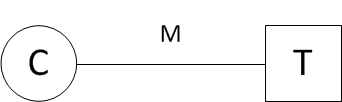
\includegraphics{06_01_basic_elements_in_contributor_thread_graph}
  \caption{The basic elements in the contributor-thread graph.}
  \label{Figure:06_01}
\end{figure}

The edges are only plotted between nodes from two disjoint sets. More precisely, there is no edge between two contributors or between two threads. As a consequence, the graph:
\[G=(V, E)\]
Where \(G\) is the graph and \(E\) is a set of edges. Especially, \(V\) is a set of nodes with the restriction of a partition:
\[V=(C \cup T)\]
And every edge in \(E\) is between \(c\) to \(t\) for some \(c\) in \(C\) and \(t\) in \(T\), so that the graph is a bipartite graph:
\[G=(C, T, E)\]
The two partitions are represented by a set of contributors and a set of threads, respectively. The edges that link the nodes refer to messages and the edge weight is denoted by the \emph{awardedpoints} attributes in \fref{Figure:06_09}. Specifically, a message labelled with zero has not been awarded any point yet.

For example, consider a contributor-thread graph shown in \fref{Figure:06_02}. The graph consists of four contributors (\(C_{1}\), \(C_{2}\), \(C_{3}\), \(C_{4}\), and \(C_{5}\)), four threads (\(T_{1}\), \(T_{2}\), \(T_{3}\), \(T_{4}\), and \(T_{5}\)), and thirteen messages. The label on the edge refers to the \emph{awardedpoints} attributes of each message. Additionally, there might be multiple edges between a contributor and a thread \((C_{1} - T_{1})\) because a contributor may post several messages to a thread.

\begin{figure}[!htb]
  \centering
  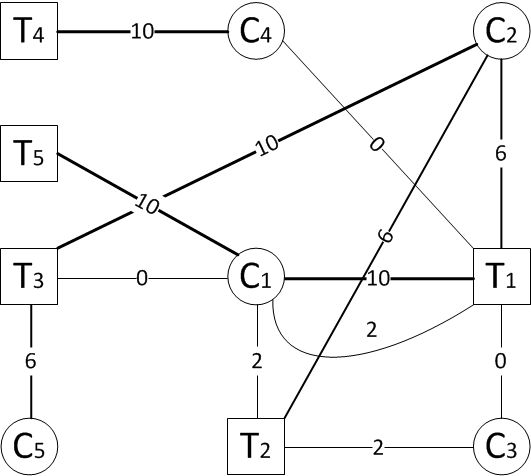
\includegraphics{06_02_sample_contributor_thread_graph}
  \caption{A sample contributor-thread graph, which contains five contributors, five threads, and thirteen messages.}
  \label{Figure:06_02}
\end{figure}

In a specific thread of the contributor-thread graph, there exist a set of contributors:
\[C_{t}=(C_{1} \cup C_{2} \cup ... \cup C_{n})\]
Where \(n > 1\), \(t\) is this thread and \(C_{t}\) is the set of contributors correspond to \(t\). \(C_{1}\) to \(C_{n}\) are contributors who have ever posted at least one awarded message (see Section~\ref{sec:data_model}) to \(t\). Hence several important terms can be defined:

\begin{enumerate}
	\item Any \(c\) in \(C_{t}\) is termed the \textbf{collaborator} on thread \(t\); \\
	\item Thread \(t\) is termed \textbf{collaborative thread}; \\
	\item Any awarded message in \(E\) which connects some \(c\) in \(C_{t}\) and \(e\) in \(E\) is termed \textbf{collaborative message}, while any other awarded message in \(E\) is termed \textbf{non-collaborative message}; \\
	\item \(C_{t}\) is termed the \textbf{collaborator set} on thread \(t\); \\
	\item When \(k = 2\), the set of all \(k\)-combinations of a set \(C_{t}\) is termed \textbf{collaboration set} and denoted by \(\binom{C_{t}}{2}\). The element in this set is named \textbf{collaborative pair}, which is a pair of collaborators on thread \(t\).

\end{enumerate}

For example, consider the thread \(T_{2}\) in \fref{Figure:06_02}. The collaborator set on collaborative thread \(T_{2}\) is made up of three collaborators \(C_{1}\), \(C_{2}\), \(C_{3}\). The collaboration set consists of three collaborative pairs \((C_{1}, C_{2})\), \((C_{1}, C_{3})\), \((C_{2}, C_{3})\). Similarly, the collaborator set on T1 contains C1 and C2 while the collaboration set consists of only one collaborative pair \((C_{1}, C_{2})\). If we consider two collaboration sets as a whole, there are three unique collaborative pairs \((C_{1}, C_{2})\), \((C_{1}, C_{3})\), \((C_{2}, C_{3})\).

\subsection{Collaborator-Thread Graph}

We impose three restraints on the contributor-thread graph \(G=(C, T, E)\) to generate the collaborator-thread graph:
\[G'=(C', T', E')\]
Where \(G'\) is the graph and \(E'\) is a set of edges. \(C'\) and \(T'\) refer to the set of collaborator nodes and thread nodes, respectively.

\begin{enumerate}
	\item \(T'\) consists of any collaborative thread in \(T\); \\
	\item \(C'\) consists of any collaborator in the union of all collaborator sets; \\
	\item \(E'\) consists of any collaborative message in \(E\).
\end{enumerate}	
	
For example, the collaborator-thread graph in \fref{Figure:06_03} is generated from the contributor-thread \fref{Figure:06_02}. \(T'\) is made up of \(T_{1}\), \(T_{2}\), and \(T_{3}\) whilst \(C'\) consists of \(C_{1}\), \(C_{2}\), \(C_{3}\), and \(C_{5}\).

\begin{figure}[!htb]
  \centering
  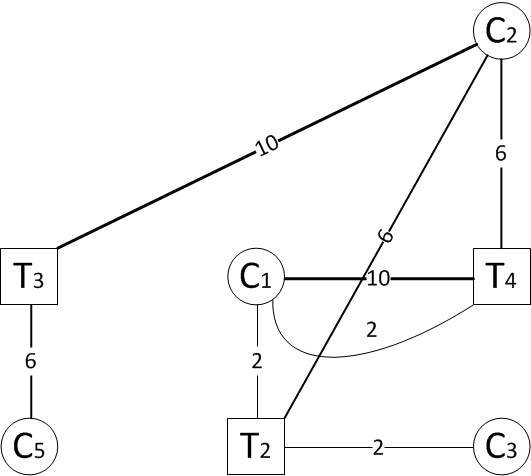
\includegraphics{06_03_sample_collaborator_thread_graph}
  \caption{The collaborator-thread graph generated from contributor-thread graph in \fref{Figure:06_02}.}
  \label{Figure:06_03}
\end{figure}

\subsection{Egocentric Collaborator-Thread Graph}

Before defining the egocentric collaborator-thread graph, we should first introduce the concept of the distance between two nodes. In graph theory, it refers to the number of edges in a shortest path linking them. For example, the distance between \(C_{1}\) and \(T_{3}\) in \fref{Figure:06_03} is three.

The following constraints can be placed on the collaborator-thread graph \(G'=(C', T', E')\) to generate an egocentric collaborator-thread graph:
\[G'_{\alpha}=(C'_{\alpha}, T'_{\alpha}, E'_{\alpha})\]
Where \(G'_{\alpha}\) is the graph and \(\alpha\) is the centric collaborator. \(E'_{\alpha}\) is a set of edges. \(C'_{\alpha}\) and \(T'_{\alpha}\) refer to the set of collaborator nodes and thread nodes, respectively.

\begin{enumerate}
	\item \(C'_{\alpha}\) includes any collaborator of distance = 2 from \(\alpha\); \\
	\item \(T'_{\alpha}\) includes any thread of distance = 1 from \(\alpha\); \\
	\item \(E'_{\alpha}\) includes any message in \(E'\) which connects some \(c\) in \(C'_{\alpha}\) and \(t\) in \(T'_{\alpha}\).
\end{enumerate}

For example, \fref{Figure:06_04} illustrates \(C_{1}\)'s collaborator-thread graph generated from the contributor-thread in \fref{Figure:06_03}. \(T'_{C_1}\) is made up of \(T_{1}\) and \(T_{2}\) whilst \(C'_{C_1}\) consists of \(C_{1}\), \(C_{2}\), and \(C_{3}\).

\begin{figure}[!htb]
  \centering
  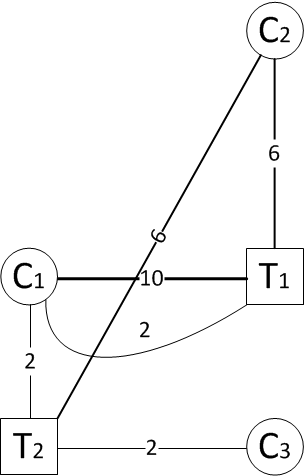
\includegraphics{06_04_sample_egocentric_collaborator_thread_graph}
  \caption{The egocentric collaborator-thread graph generated from collaborator-thread graph in \fref{Figure:06_03}.}
  \label{Figure:06_04}
\end{figure}

\subsection{Collaborative Graph}

The collaborative graph is a single-edge, undirected, and weighted graph, which is generated from the collaborator-thread graph. It shows an indirect relation between collaborators. In other words, one collaborator is connected to another because they have posted awarded messages to the same thread, although they may not have replied to each other.

As described in Section~\ref{sec:contributor_thread_graph}, the relation between two collaborators in the collaborator set is termed collaborative pair. Compared with the pairs that have only collaborated once, the pairs who have collaborated many of the same thread have a closer link. Therefore the weight of a collaborative pair is denoted by the number of collaborative threads it belongs to.

Given a collaborator-thread graph \(G'=(C', T', E')\), the collaborative graph:
\[G''=(V'', E''))\]
Where \(G''\) is the graph and \(E''\) is a set of edges. \(V''\) refers to the set of nodes.

\begin{enumerate}
	\item \(V''\) consists of any collaborator in \(C'\); \\
	\item \(E''\) consists of any collaborative pair in the union of all collaboration sets. The edge weight is denoted by the number of collaborative thread this collaborative pair belongs to.
\end{enumerate}

Take the collaborator-thread graph in \fref{Figure:06_03} for example. According to the definition, we should first find out all collaborators as the nodes and all collaborative pairs as the edges. As shown in \fref{Figure:06_05}, the graph is made up of four collaborators (\(C_{1}\), \(C_{2}\), \(C_{3}\), and \(C_{5}\)) as well as four edges plotted among them. The edge weight of (\(E_{12}\) is two because this collaborative pair belongs to two collaborative threads (\(T_{1}\) and \(T_{2}\)), while other edges including (\(E_{13}\), (\(E_{23}\), and (\(E_{25}\) are all weighted with one.

\begin{figure}[!htb]
  \centering
  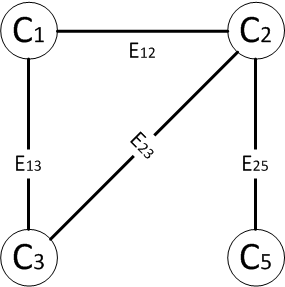
\includegraphics{06_05_sample_collaborative_graph}
  \caption{The collaborative graph generated from the collaborator-thread graph in \fref{Figure:06_03}.}
  \label{Figure:06_05}
\end{figure}

\subsection{Metrics of Collaborative Graph} \label{sec:collaborative_graph_metrics}

This section defines several metrics of the collaborative graph, which will be mapped to diverse visual properties of the collaborative graph visualisation.

\textbf{Contribution.}~The contribution refers to the sum of points a collaborator has ever been awarded in the snapshot. As discussed in Section~\ref{sec:tech_desc}, the contribution represents the expertise of a specific contributor in the snapshot. There are four interconnected measures of contribution. The first two metrics are related to individuals while the last two metrics reflect the community nature. The sum of the first two metrics is termed individual contribution, and the sum of the last two metrics is termed community contribution. The collaborative contribution (individual) which is the accumulated points earned from all collaborative messages, and non-collaborative contribution (individual) which is the accumulated points gained from all non-collaborative messages. In contrast to the contribution which has been awarded to individuals, the sum of all collaborative contribution (individual) is named by the collaborative contribution (community), whilst the sum of all non-collaborative contribution (individual) is termed the non-collaborative contribution (community).

\textbf{Risk Attributes.}~In the \emph{Risk Assessment} use case (see U3 in Section~\ref{sec:use_cases}), the risk of experts leaving has been analysed in the aspects of the risk impact and likelihood (see R2 in Section~\ref{sec:requirements}). Having introduced four measures of the contribution, it is easy to define these two metrics. More precisely, the likelihood attribute refers to the ratio of the individual contribution to community contribution. The impact attribute is denoted by the ratio between non-collaborative contribution to contribution. \fref{Figure:06_06} presents the likelihood and impact of each contributor as well as the above-mentioned contribution metrics based on the collaborative graph shown in \fref{Figure:06_05}.

\begin{figure}[!htb]
  \centering
  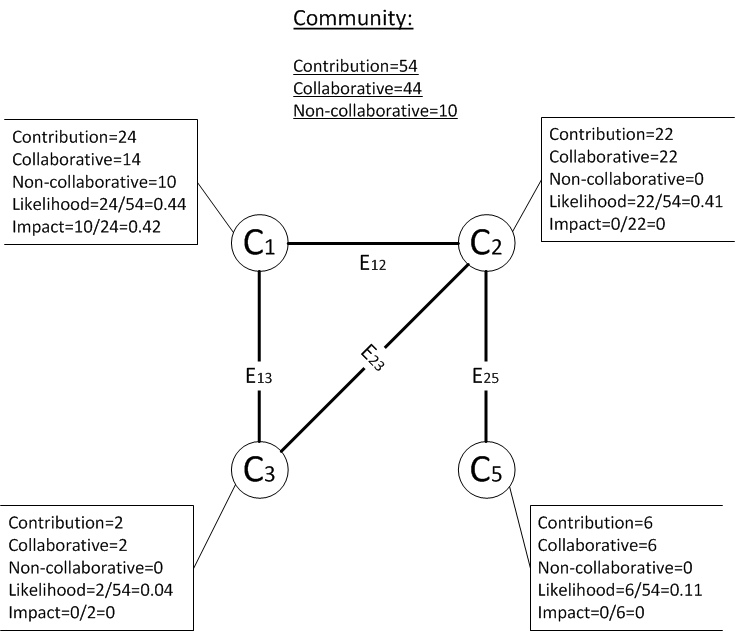
\includegraphics[width=13cm]{06_06_sample_collaborative_graph_likelihood_impact}
  \caption{The contribution, likelihood, and impact metrics in the sample collaborative graph.}
  \label{Figure:06_06}
\end{figure}

\textbf{Degree Centrality.}~The degree centrality is the total number of edges connected to a particular node, which determines the relative importance of a node in the graph. This metric identifies collaborators that actively collaborate or collaborators through which flows most of the expertise. Both are critical members of the forum because their leaving may limit the exchange of expertise. However, this metric does not differentiate between quantity and quality. Take the collaborative graph in \fref{Figure:06_05} for example, the degree centrality of \(C_{2}\) is three, but it does not recognize the difference between a link to the \(C_{1}\) whose contribution is 24 points and a link to \(C_{5}\) whose contribution is only 2 points.

\textbf{Betweenness Centrality}~The betweenness centrality labels each node with a value which is the number of shortest paths that pass through it. Take the collaborative graph in \fref{Figure:06_05} for example, there are two shortest paths that pass through \(C_{2}\) (\(E_{12}\)-\(E_{25}\) and \(E_{23}\)-\(E_{25}\)), thus the betweenness centrality of \(C_{2}\) is two. Especially, this measure can be also applied to an edge that represents a collaborative pair in the collaborative graph. The edge betweenness of \(E_{25}\) in \fref{Figure:06_05} is three because there are three shortest paths pass through it \(E_{25}\), \(E_{12}\)-\(E_{25}\), and \(E_{23}\)-\(E_{25}\). \fref{Figure:06_07} presents the degree centrality and node betweenness centrality as well as the edge betweenness centrality of the collaborative graph shown in \fref{Figure:06_05}.

\begin{figure}[!htb]
  \centering
  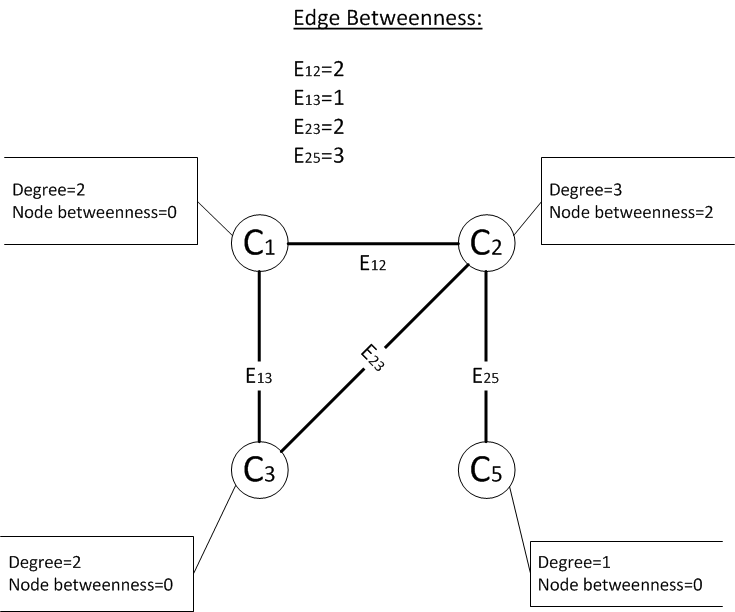
\includegraphics[width=13cm]{06_07_sample_collaborative_graph_degree_betweenness}
  \caption{The degree centrality, node betweenness centrality, and edge betweenness centrality in the sample collaborative graph.}
  \label{Figure:06_07}
\end{figure}

Within graph theory, the bridge is a special type of edge that would divide the whole graph into several disjoint subgroups if it was removed. In the collaborative graph, consider again the edge that represents the collaborative pair, the edges with a high betweenness centrality play a vital role because they act as the bridge to connect separated subgroups. Hence, the concept of edge betweenness centrality will be used in the cluster finding algorithm which is detailed in Section~\ref{Section:WGN}.

\subsection{Weighted Girvan-Newman Algorithm} \label{Section:WGN}

The cluster finding algorithms have been widely proposed in the literature to detect subgroups. Although most of them are specifically designed for unweighted graphs, some others can be also used in weighted graphs. For example, when the edge weight is taken into account, the Weighted Girvan-Newman algorithm \citep{Newman2004} simply add an extra step of division by the weight of the corresponding edge based on the original Girvan-Newman algorithm \citep{Girvan2002}. The idea of the Weighted Girvan-Newman algorithm can be briefly described as follows:
\begin{enumerate}
	\item Calculate the edge betweenness of all edges in the graph; \\
	\item Divide each edge betweenness by the corresponding edge weight. This result is termed generalised edge betweenness; \\
	\item Remove the edge with the highest generalised edge betweenness to form a new graph. Especially, if multiple edges have the same generalised edge betweenness, remove any of them; \\
	\item Check if there exists any edge in the new graph. If yes then go to step 1, if no then end the algorithm.
\end{enumerate}

\fref{Figure:06_08} presents the detailed process of the Weighted Girvan-Newman algorithm based on the collaborative graph in \fref{Figure:06_05}.

\begin{figure}[!htb]
  \centering
  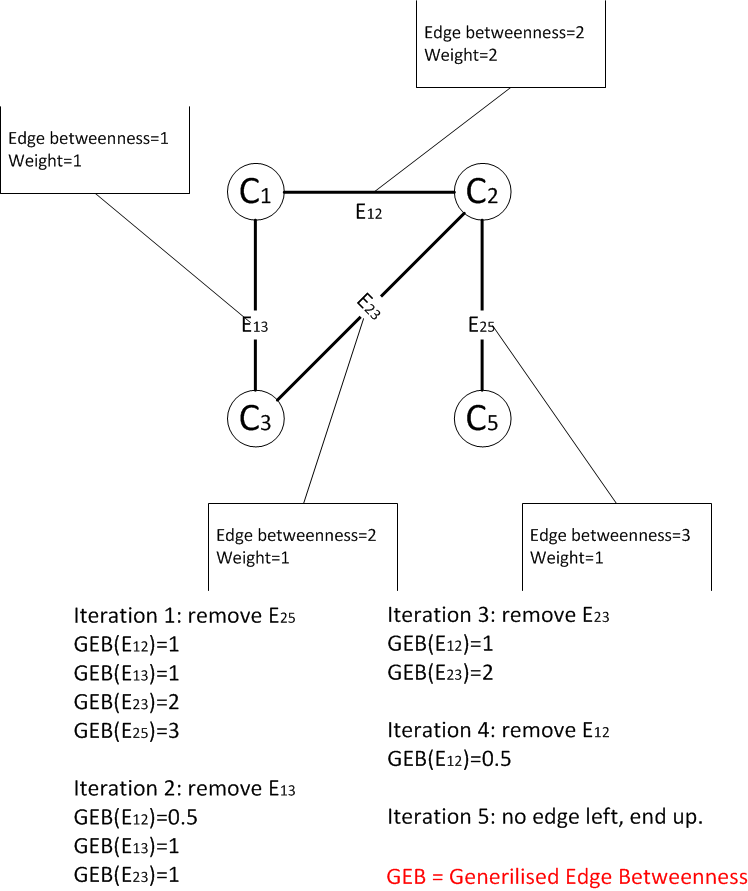
\includegraphics[width=13cm]{06_08_sample_collaborative_graph_weighted_girvan_newman_algorithm}
  \caption{The Weighted Girvan-Newman algorithm in the sample collaborative graph.}
  \label{Figure:06_08}
\end{figure}

\subsection{Visual Properties of Collaborative Graph} \label{sec:collaborative_graph_visual_props}

The visual properties play a crucial role in the node-edge diagram, which includes the node size, node colour, node opacity, node label, edge thickness, and edge colour.

\textbf{Node Size.}~In the collaborative graph, the node size represents the importance of the collaborator in the graph from three different aspects: the contribution, degree centrality, and betweenness centrality (see Section~\ref{sec:collaborative_graph_metrics}). When posting multiple awarded messages, a contributor can be awarded more than 10 points in a single thread. In this case, a contributor who gained all message points only from a single thread may be the highest in the graph. But we cannot definitely infer this contributor is the most important individual, because we should take the centrality metrics into account. For example, if the node size is mapped to the degree centrality, the node with the maximum degree has the biggest size in the graph. By default, it is mapped to the contribution of the collaborator:

\[S(v)=S_{min} + \frac{(S_{max} - S_{min}) \times P(v)}{P_{max}}\]

Where \(v\) is any node in the graph and \(S(v)\) is the node size of \(v\). \(S_{max}\) and \(S_{min}\) are the biggest and smallest node size. \(P_{max}\) is the maximum contribution in the graph and \(P(v)\) is the contribution of \(v\). For example, consider the collaborative graph in \fref{Figure:06_05}:

\[S(C_{1})=8 + \frac{50 \times 14}{22}=40 \quad \quad S(C_{2})=8 + \frac{50 \times 22}{22}=58\]
\[S(C_{3})=8 + \frac{50 \times 2}{22}=13 \quad \quad S(C_{5})=8 + \frac{50 \times 6}{22}=22\]

Where \(S_{min} = 8\) and \(S_{max} = 58\). Similarly, the node size based on other metrics:

\[S(v)=S_{min} + \frac{(S_{max} - S_{min}) \times D(v)}{D_{max}}\]
\[S(v)=S_{min} + \frac{(S_{max} - S_{min}) \times B(v)}{B_{max}}\]

Where \(D_{max}\) is the maximum degree centrality while \(B_{max}\) is the maximum betweenness centrality. \(D(v)\) and \(B(v)\) are the degree centrality and betweenness centrality of \(v\), respectively.

\textbf{Node Colour.}~The colour of each node is mapped to the risk impact attribute, which ranges from 0 to 1. Four different colours are provided to visualise this metric:

\[C(v) = \left\{\begin{array}{l l}
    RGB(255,0,0) \quad \quad 0.75 < I(v) < 1\\
    RGB(255,165,0) \quad \quad 0.5 < I(v) \leq 0.75\\
    RGB(255,255,0) \quad \quad 0.25 < I(v) \leq 0.5\\
    RGB(0,255,0) \quad \quad 0 < I(v) \leq 0.25
  \end{array} \right.
\]

Where \(v\) is any node in the graph and \(C(v)\) is the node colour of \(v\) in the form of RGB code. \(I(v)\) is the risk impact of \(v\). For example, consider the collaborative graph in \fref{Figure:06_05}:

\[C(C_{1})=RGB(255,255,0) \quad \quad C(C_{2})=RGB(0,255,0)\]
\[C(C_{3})=RGB(0,255,0) \quad \quad C(C_{5})=RGB(0,255,0)\]

\textbf{Node Opacity.}~The opacity of each node is mapped to the risk likelihood attribute, which also ranges from 0 to 1. With the purpose of ensuring each node is visible, the minimum opacity is expected to be taken into account:

\[O(v)=O_{min} + \frac{(o_{max} - O_{min}) \times L(v)}{O_{max}}\]

Where \(v\) is any node in the graph and \(O(v)\) is the node opacity of \(v\). \(O_{max}\) and \(O_{min}\) are the highest and lowest node opacity. \(L(v)\) is the risk likelihood of \(v\). For example, consider the collaborative graph in \fref{Figure:06_05}:

\[O(C_{1})=0.5 + \frac{0.5 \times 0.44}{1}=0.77 \quad \quad O(C_{2})=0.5 + \frac{0.5 \times 0.41}{1}=0.71\]
\[O(C_{3})=0.5 + \frac{0.5 \times 0.04}{1}=0.52 \quad \quad O(C_{5})=0.5 + \frac{0.5 \times 0.11}{1}=0.56\]

Where \(O_{max} = 1\) and \(O_{min} = 0.5\).

\textbf{Node Label.}~The label of nodes displays the \emph{contributor} attribute of the \emph{Contributor} class (see Section~\ref{sec:data_model}). The label visibility is determined by the node size, which is configurable in the visual properties panel in the graph options window (see Section~\ref{sec:collaborative_graph_options_window}).

\textbf{Edge Thickness.}~The thickness of edges indicates to what extend a collaborator pair has the similar expertise, or how tightly they connect with. By default, it is mapped to the edge weight:

\[T(e)=T_{min} + \frac{(T_{max} - T_{min}) \times W(e)}{W_{max}}\]

Where \(e\) is any edge in the graph and \(T(e)\) is the edge thickness of \(e\). \(T_{max}\) and \(T_{min}\) are the biggest and smallest edge thickness. \(W_{max}\) is the maximum edge weight in the graph and \(W(e)\) is the edge weight of \(e\). For example, consider the graph in \fref{Figure:06_05}:

\[T(E_{12})=1 + \frac{4 \times 2}{2}=5 \quad \quad T(E_{13})=1 + \frac{4 \times 1}{2}=3\]
\[T(E_{23})=1 + \frac{4 \times 1}{2}=3 \quad \quad T(E_{25})=1 + \frac{4 \times 1}{2}=3\]

Where \(T_{max} = 5\) and \(T_{min} = 1\).

\textbf{Edge Colour.}~The colour of nodes is preserved for the use of highlighting and clustering. By default, the node colour is light grey.

\subsection{Visual Properties of Collaborator-Thread Graph}
Similar to the collaborative network, there are two visual properties in the collaborator-thread graph.

\textbf{Node Icon.}~Since there are two distinct nodes in the graph, two icons is used to distinguish the collaborator node and thread node.

\textbf{Edge Thickness.}~The edge thickness is mapped to the awarded points of the message:

\[T(e) = \left\{\begin{array}{l l}
    1 \quad \quad P(e) = 2\\
    2 \quad \quad P(e) = 6\\
    4 \quad \quad P(e) = 10
  \end{array} \right.
\]

Where \(e\) is any edge in the graph and \(T(e)\) is the edge thickness of \(e\). \(P(e)\) is the awarded points of \(e\).

\subsection{Enhanced Data Model}

\fref{Figure:06_09} shows the enhanced class diagram based on the tailored data model (see \fref{Figure:05_02}) by adding several concepts introduced in Section~\ref{sec:contributor_thread_graph}.
 
In the centre of the diagram, the \emph{CollaborativeThread} class is a subclass of the \emph{Thread} class, which contains at least one instance of the \emph{CollaborativePair} class. For each collaborative pair, it contains exactly two distinct instance of the Collaborator class. In addition, there is an attribute \emph{amount} to indicate the number of collaborative thread it belongs to. The constraints on the \emph{Collaborator} class are that any instance in this class is also an instance of the Contributor class and must belong to at least one collaborative pair.

Now we can realise the collaborator-thread graph as well as the collaborative graph more clearly with the help of \fref{Figure:06_09}. The collaborator node and thread node of the collaborator-thread graph are actually the \emph{Collaborator} class and the \emph{CollaborativeThread} class, respectively. The edges of the collaborator-thread graph consist of any instance in the \emph{AwardedMessage} class which is posted by a collaborator. The edge weight is the \emph{awardedpoints} attribute. Similarly, the node and edge of the collaborative graph refer to the \emph{Collaborator} and \emph{CollaborativePair} class, respectively. The edge weight is the \emph{amount} attribute.

\begin{figure}[!htb]
  \centering
  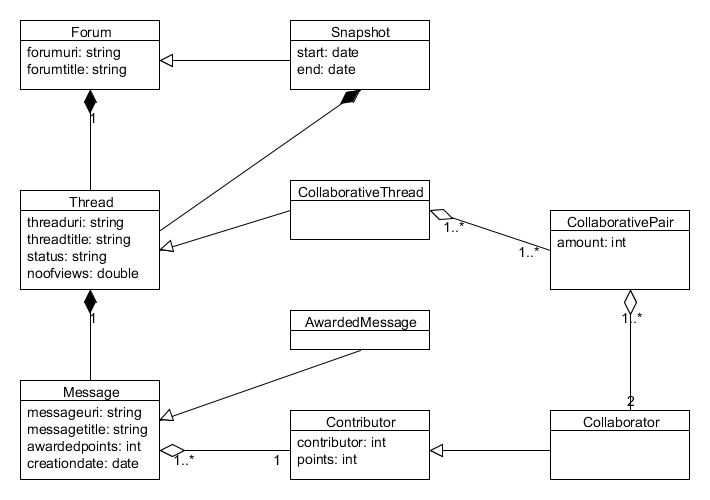
\includegraphics[width=13cm]{06_09_enhanced_class_diagram}
  \caption{The enhanced data model by adding basic concepts for the forum visualisation tool.}
  \label{Figure:06_09}
\end{figure}

\fref{Figure:06_10} shows a sample object diagram generated from the contributor-thread graph in \fref{Figure:06_02}. The instances in grey are excluded from the collaborator-thread graph. The object t4 in the bottom left of the diagram is not a collaborative thread because it does not contain any object of the \emph{CollaborativePair} class. The object m4, m5, and m9 are not objects of the \emph{AwardedMessage} class because they have not been awarded any point. Especially, the object m12 in the bottom centre of the diagram is awarded ten points. But it is posted by c4 who is not an object of the \emph{Collaborator} class. The object c4 is not an object of the \emph{Collaborator} class because it does not belong to any instance of the \emph{CollaborativePair} class. In the collaborative graph, the object cp1 is an edge between two objects c1 and c2 with the weight two because cp1 belongs to two distinct threads t1 and t2.

\begin{figure}[!htb]
  \centering
  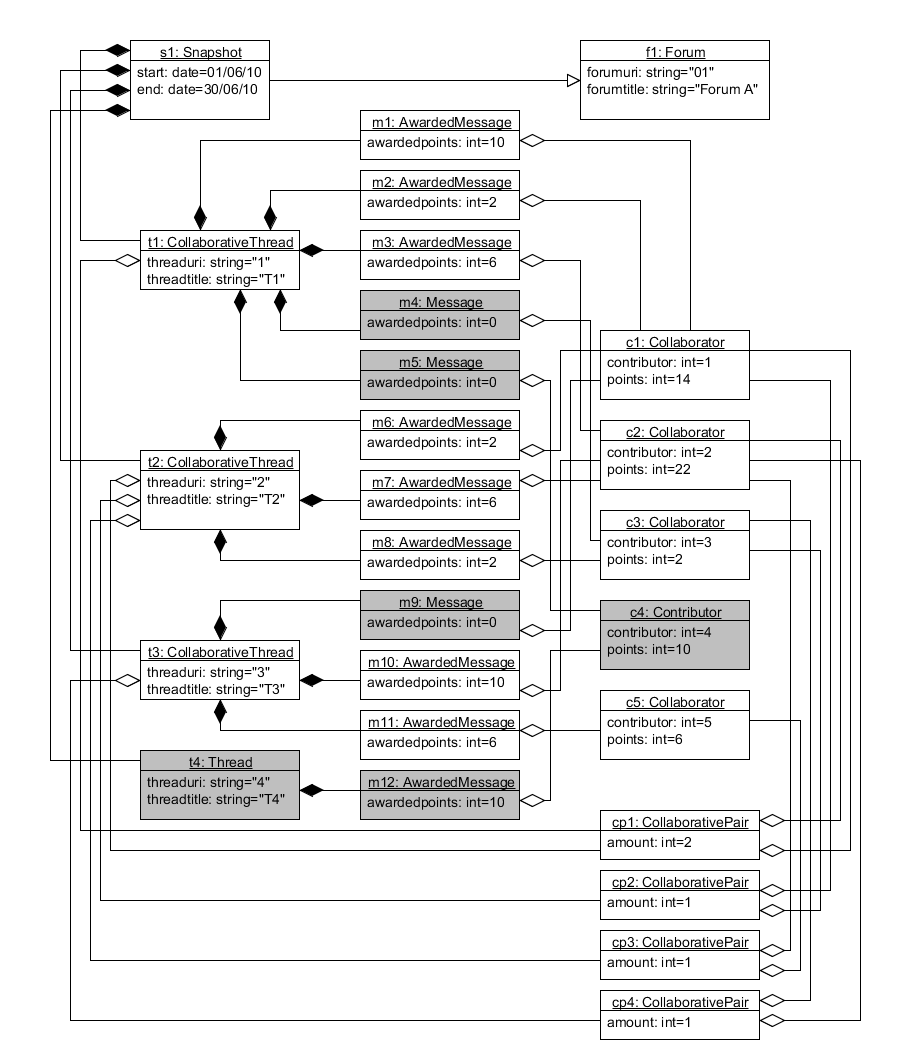
\includegraphics[width=13cm]{06_10_sample_object_diagram}
  \caption{The sample object diagram generated from the contributor-thread graph in \fref{Figure:06_02}.}
  \label{Figure:06_10}
\end{figure}

\section{User Interface Design}

In Section~\ref{sec:requirements}, R2 and R3 have imposed two requirements in the the collaborative graph and egocentric collaborator-thread graph, respectively. Section~\ref{sec:graph_design} have already defined these two graphs as well as their metrics and visual properties.
This section describes the user interface design of the corresponding graph visualisations. Added to that, the snapshot explorer will be also depicted.

\subsection{Snapshot Explorer}

The snapshot is not explicitly mentioned in the use case scenario discussed in Section~\ref{sec:requirements}. However it is still an indispensable component in the forum visualisation tool for two reasons. Firstly, the condition panel provides the user interface to collect the input of the \emph{Load Snapshot} use case (see U1 in Section~\ref{sec:use_cases}). Secondly, the tree view and properties window allow end users to browse the snapshot data in the traditional hierarchical structure, while the properties window displays detailed information of items in the tree view. The former has a mutual link with the main window of the collaborator-thread graph. The latter will be invoked by the main window of both collaborative graph and collaborator-thread graph. \fref{Figure:06_11} shows the main window of the snapshot explorer which consists of the conditions panel and tree view.

\begin{figure}[!htb]
  \centering
  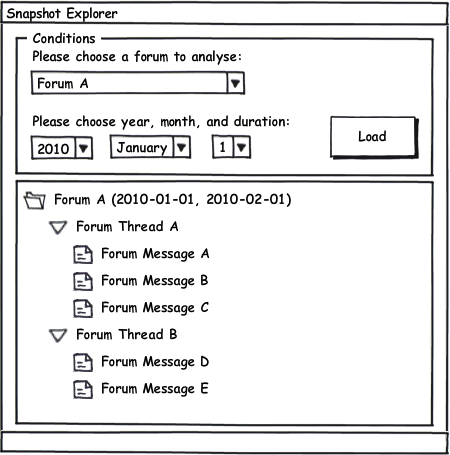
\includegraphics[width=8cm]{06_11_snapshot_explorer_main_window}
  \caption{The main window of the snapshot explorer.}
  \label{Figure:06_11}
\end{figure}

\subsubsection{Conditions Panel}

As mentioned in the previous chapter, a snapshot is uniquely identified by the forum and a given period of time. In the conditions panel, the end users choose a forum in the drop-down list, then select the year, month, and duration to calculate the \emph{start} and \emph{end} attributes in the \emph{Snapshot} class. When clicking the Load button, a long-running cancellable task will be established in a background thread without blocking the user interface. Meanwhile, the Load button is set to disabled to guarantee there is only one task running at a time. Once the data has been loaded from the data source, the new snapshot data will be added into the tree view, and the Load button is set to enable again. In addition, the collaborative graph of this snapshot will be automatically opened in a new window.

\subsubsection{Tree View}
The tree view provides a tri-level hierarchical structure to display the snapshot data. The top level nodes represent an object of the \emph{Snapshot} class, while the second level nodes and the leaf node refer to an instance of the \emph{Thread} and \emph{Message} class, respectively. When double-clicking a particular node, the detailed information will be displayed in the properties window.

\subsubsection{Properties Window}
The properties window simply makes use of the key-value pair to list all attributes of an entity defined in the data model. \fref{Figure:06_12} presents the properties window of an object of the \emph{Thread} class.

\begin{figure}[!htb]
  \centering
  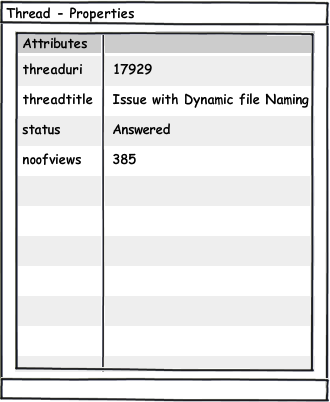
\includegraphics[width=8cm]{06_12_snapshot_explorer_properties_window}
  \caption{The properties window of the snapshot explorer.}
  \label{Figure:06_12}
\end{figure}

\subsection{Collaborative Graph Visualisation}
In this section, the user interface design of the collaborative graph visualisation will be depicted which including the main window (Section~\ref{sec:collaborative_graph_main_window}), dynamic filters window (Section~\ref{sec:collaborative_graph_filters_window}), and graph options window (Section~\ref{sec:collaborative_graph_options_window}). Additionally, the highlighting mechanism (Section~\ref{sec:collaborative_graph_highlighting}) which plays an important role in both main window and graph options window will be described in more details.

\subsubsection{Main Window} \label{sec:collaborative_graph_main_window}
\fref{Figure:06_13} presents the main window of the collaborative graph, which consists of the master view, satellite view and toolbar. The master view is the main part of the visualisation, while the satellite view on the whole or large part of the graph contains a lens shape that shows the boundaries of the visible part of the graph in the master view. The tool bar provides commonly used functionalities. The master view of the collaborative graph provides several dynamic functionalities and most of them take place via a mouse:

\begin{enumerate}
	\item Scale the whole graph with the scroll wheel or with the `Zoom In' or `Zoom Out' buttons in the toolbar; \\
	\item Fit to view by clicking the `Fit to View' button in the toolbar when the master view is too big to have an overview or too small to see details; \\
	\item Pan the whole graph by dragging the mouse in the move mode, or move around a set of nodes after selecting them by clicking on them or dragging a rectangle around them in the select mode. Add to that, multiple nodes can be also picked by holding the shift key. Two modes can be switched by clicking the `Select' or `Move' toggle buttons in the toolbar; \\
	\item Show or hide the satellite view by clicking the `Satellite' button in the toolbar; \\
	\item Show detailed information in tooltip when hovering over nodes or edges. For nodes, the information includes the \emph{contributor} and \emph{points} attributes of the \emph{Contributor} class, as well as graph metrics (e.g. degree centrality) on the fly. For edges, the information includes the \emph{amount} attribute of the \emph{CollaborativePair} class; \\
  \item Show detailed information in the properties window (see \fref{Figure:06_12}) in the context menu of nodes or edges; \\
	\item Link to the collaborator-thread graph when selecting the corresponding menu item in the context menu of nodes.
\end{enumerate}

\begin{figure}[!htb]
  \centering
  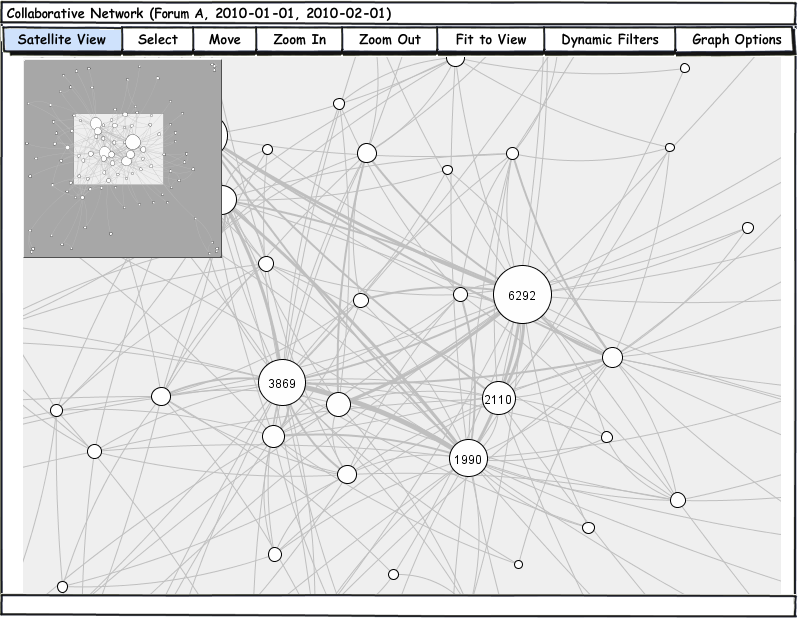
\includegraphics[width=13cm]{06_13_collaborative_graph_main_window}
  \caption{The main window of the collaborative graph.}
  \label{Figure:06_13}
\end{figure}

Based on the same model, the above interactions affect the master view as well as the lens shape in the satellite view. In addition, the visual properties in Section~\ref{sec:collaborative_graph_visual_props} are applied to both views.

\subsubsection{Highlighting} \label{sec:collaborative_graph_highlighting}

It is common to provide highlighting mechanism in the graph visualisation. Vizster \citep{Heer2005a} makes use of highlighting to annotate all friends of a specific user within a social network. By contrast, Invenio \citep{Singh2007} utilises the highlighting feature to mark different node sets in a multi-modal graph. In the collaborative graph visualisation, highlighting plays an important role in two scenarios. Firstly, when a set of nodes has been picked in the select mode, all picked nodes will be rendered in yellow. Their neighbour nodes are expected to be highlighted in red, as well as the edges that are plotted between any node in the picked node set and neighbour nodes. This feature is particularly useful in a large-scale graph as shown in \fref{Figure:06_14}, which clearly indicates all neighbour node of a set of picked nodes. Secondly, when cluster finding feature is on, each subgroup will be highlighted with a random colour which will be detailed described in the following section.

\begin{figure}[!htb]
  \centering
  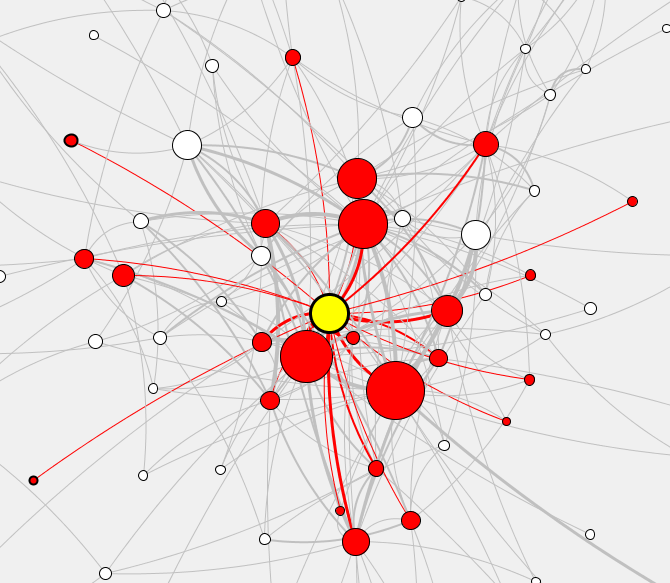
\includegraphics[width=13cm]{06_14_highlighting_neighbour_nodes}
  \caption{The highlighting mechanism is used to mark neighbour nodes}
  \label{Figure:06_14}
\end{figure}

\subsubsection{Dynamic Filters Window} \label{sec:collaborative_graph_filters_window}

The filtering mechanism provides a way to remove a set of nodes and/or edges under a given set of conditions from the dual-view of the collaborative graph visualisation. As shown in \fref{Figure:06_15}, there are two panels in the dynamic filters window: node filters panel and edge filters panel.

The node filters panel consists of three metrics: contribution, degree centrality, and betweenness centrality (see Section~\ref{sec:collaborative_graph_metrics}). For each metric, a slider from zero to maximum is provided to adjust the threshold value which is displayed in the red label above each slider. When dragging the slider knob, the corresponding threshold value is also changed to remove all elements whose metric is less than the threshold value from the dual-view. For example, if the threshold value of the contribution slider is set to 100. That means any nodes whose contribution is less than 100 will be filtered out from dual-view of the collaborative graph visualisation. Moreover, if the threshold value of the contribution slider reaches the maximum, only the node with the highest contribution appears in the dual-view. Similarly, the edge filters panel is made up of the number of the collaborative thread, which is also the edge weight. Additionally, multiple aforementioned metrics can be combined to form a compound condition.

\begin{figure}[!htb]
  \centering
  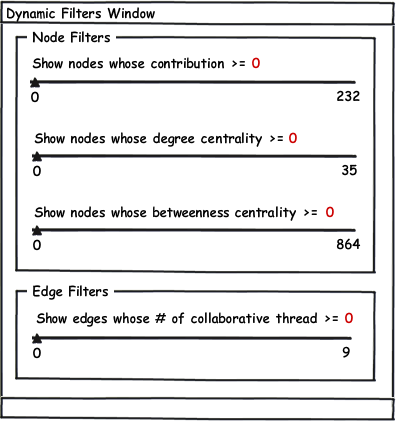
\includegraphics[width=8cm]{06_15_collaborative_graph_dynamic_filters_window}
  \caption{The dynamic filter window of the collaborative graph visualisation.}
  \label{Figure:06_15}
\end{figure}

\subsubsection{Graph Options Window} \label{sec:collaborative_graph_options_window}
\fref{Figure:06_16} presents the graph options window of the collaborative graph visualisation, which can be divided into two sub-components: the cluster finding panel and the visual properties panel.

\begin{figure}[!htb]
  \centering
  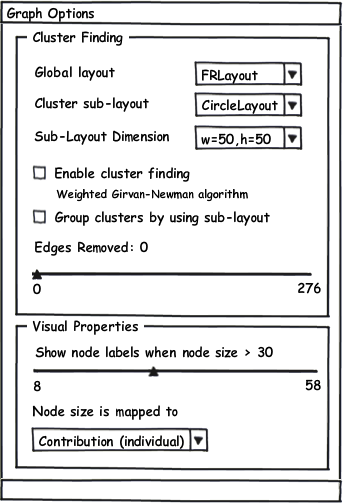
\includegraphics[width=8cm]{06_16_collaborative_graph_visualisation_graph_options_window}
  \caption{The graph options window of collaborative graph visualisation.}
  \label{Figure:06_16}
\end{figure}

\textbf{Cluster Finding Panel.}~The layout algorithm is in charge of calculating the coordinate of each node. The global layout drop-down list provides a way for end users to switch the global layout displayed in both the master view and satellite view. By default, the global layout is set to Fruchterman-Reingo \citep{Fruchterman1991} since two collaborators connected with an edge that has a higher weight will be plotted much closer, in order to indicate they have more similar knowledge.

The enable cluster finding checkbox acts as an on-off switch to start and stop the clustering mechanism. When this checkbox has been selected, the edges removed slider is set to enable. The value of this slider is mapped to a threshold which determines the number of iteration in the Weighted Girvan-Newman algorithm discussed in Section~\ref{Section:WGN}. For each subgroup in the new graph generated by the algorithm, a set of random colours is expected to highlight different subgroups so that all nodes in the same group will be rendered the same colour.

Additionally, the group cluster drop-down list provides an option for end users to establish a sub-layout for each subgroup in order to gather all nodes in the same subgroup around a small region. When this drop-down list has been selected, the cluster sub-layout drop-down list can be used to change the sub-layout of all subgroups, while the sub-layout dimension drop-down list determines the size of the small region which contains all elements of the subgroup.

\textbf{Visual Properties Panel.}~The visual properties panel provides two features to configure the node label as well as the node size. The show node labels slider allows end users to input a threshold value to make any node whose node size is greater than the threshold visible. The node size is mapped to drop-down list can be used to change the metric which is mapped to the node size. Once the option of this list has been change, the master and satellite view will be immediately refreshed to display the new view.

\subsection{Collaborator-Thread Graph Visualisation}
In this section, the user interface design of the collaborator-thread graph visualisation will be depicted which including the main window (\ref{sec:c_t_graph_main_window}) and temporal chart window (\ref{sec:c_t_graph_temporal_chart_window}).

\subsubsection{Main Window} \label{sec:c_t_graph_main_window}
\fref{Figure:06_17} presents the main window of the collaborator-thread graph visualisation, which is much the same the main window of the collaborative graph visualisation.

\begin{figure}[!htb]
  \centering
  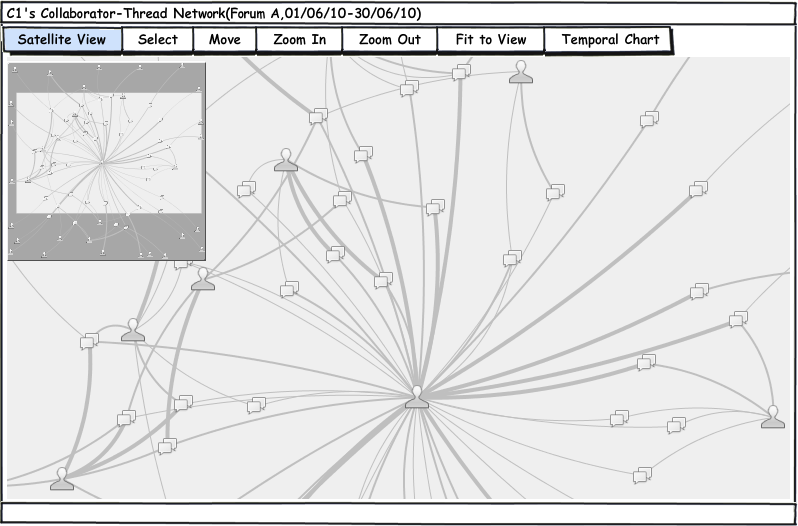
\includegraphics[width=13cm]{06_17_collaborator_thread_graph_visualisation_main_window}
  \caption{The main window of collaborator-thread graph visualisation.}
  \label{Figure:06_17}
\end{figure}

\subsubsection{Temporal Chart Window} \label{sec:c_t_graph_temporal_chart_window}
The collaborator-thread graph visualisation provides time-dependant functionalities for the risk manager to see and compare the changes over time including the risk likelihood and impact. As shown in \fref{Figure:06_18}, the temporal chart window is made up of three major components: the bar chart, the timeline slider, and the metric drop-down list.

\begin{figure}[!htb]
  \centering
  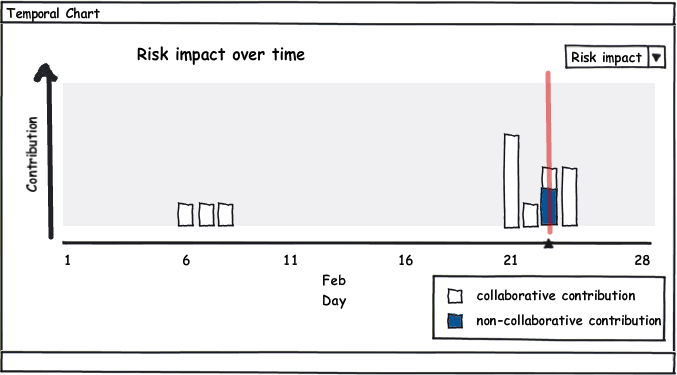
\includegraphics[width=13cm]{06_18_collaborator_thread_graph_visualisation_temporal_chart_window}
  \caption{The temporal chart window of collaborator-thread graph visualisation.}
  \label{Figure:06_18}
\end{figure}

Users are allowed to use the timeline slider to navigate through different time points by dragging the slider knob to see the evolution of the snapshot. Above the timeline slider, a bar chart shows how risk likelihood or impact changes over time, which enables users to see several important metrics during navigations. The metric drop-down list allows users to observe different metrics in the bar chart.

\section{Summary}
This chapter first defines two types of graphs: the collaborative graph and egocentric collaborator-thread graph. Then the graph metrics and corresponding visual properties have been added into the collaborative graph. Lastly, the user interface design of three major components in the forum visualisation tool have been described.
